\section{Procedure}
\label{sec:procedure}
The following part describes the experimental set up and procedure. It is based on the given
instructions and has been modified to the actual procedure in the lab.

\subsection{Measuring the speed of light through phase differences}
\label{sec:measuring}
\begin{figure*}
    \centering
    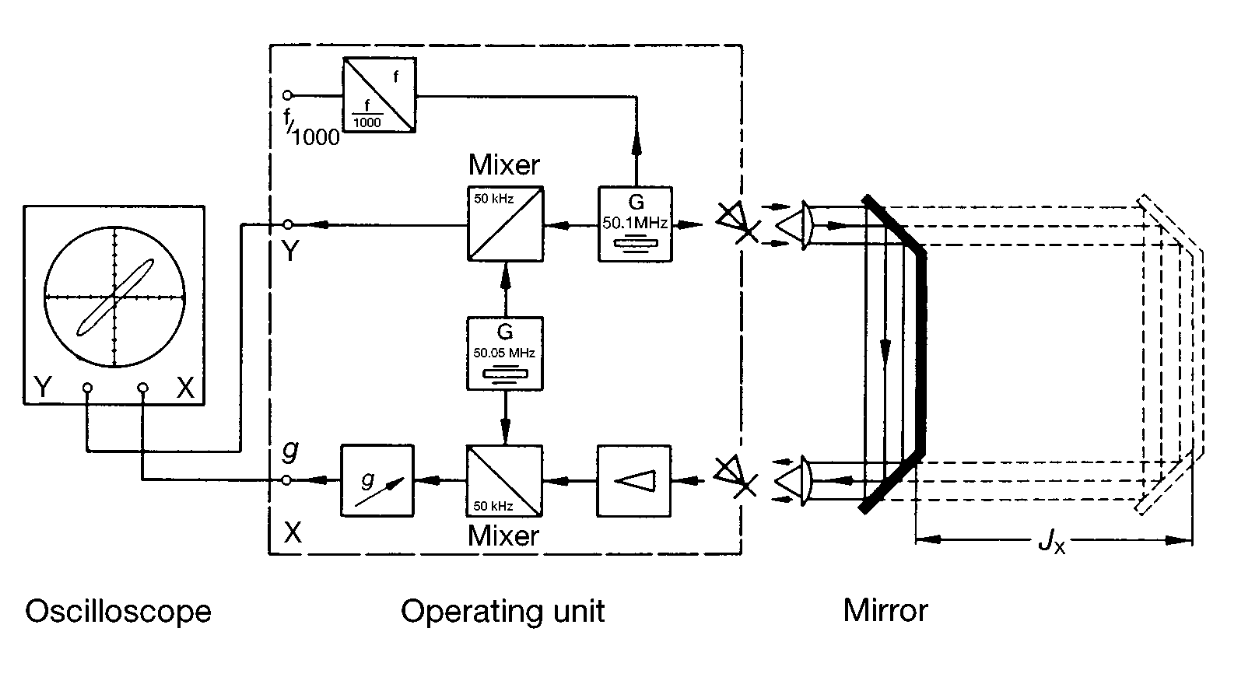
\includegraphics[width=0.8\textwidth]{media/Setup Air.png}
    \caption{Diagram of the experimental set-up for measuring the velocity of light in air
              \cite{LabInstructions}.}
    \label{fig:SetupAir}
\end{figure*}
To measure the speed of light in air, a setup as shown in \autoref{fig:SetupAir} is used. A source
of modulated light and a detector is sending a light pulse towards a mirror set up where it gets
reflected to the detector unit. An oscilloscope attached to the operating unit shows a Lissajous
figure corresponing to the phase difference between sent light and received signal.

For each measurement, the distance between the mirror and operating unit gets extended by
\[
\Delta x
\]
resulting in an extra light path
\[
  \Delta l = 2 \Delta x.
\]
$\Delta x$ is chosen such that a phase change of $\pi / 2$ is added. The originally intended $\pi$
were not possible as the light sourse lost its definition after $\Delta x \gtrapprox \SI{1}{m}$).

To travel $\Delta l$, the light needs 
\[
  \Delta t = \frac{1}{4f}
\]
with the \textit{modulation frequency} $f = \SI{50.1}{MHz}$. Since
\[
  \text{Speed} = \frac{\text{Distance}}{\text{Time}},
\]
we can conclude that
\[
  c = \frac{\Delta l}{\Delta t} = 8f \Delta x.
\]


